\documentclass[aspectratio=169,11pt]{beamer}

% ----------------------------------------------------------------------------
%  Balíčky a kódování
% ----------------------------------------------------------------------------
\usepackage[T1]{fontenc}
\usepackage[utf8]{inputenc}
\usepackage{lmodern}
\usepackage{amsmath,amssymb}
\usepackage{textcomp}
\usepackage{booktabs}
\usepackage{tikz}
\usetikzlibrary{positioning,arrows.meta}

% ----------------------------------------------------------------------------
%  Barevné schéma a téma
% ----------------------------------------------------------------------------
\usetheme{Madrid}
\usecolortheme{default}

\definecolor{grassdark}{RGB}{27,94,32}
\definecolor{grassmid}{RGB}{56,142,60}
\definecolor{grasslight}{RGB}{232,245,233}
\definecolor{alertred}{RGB}{183,28,28}
\definecolor{alertlight}{RGB}{255,235,238}
\definecolor{slate}{RGB}{55,71,79}
\definecolor{slatelight}{RGB}{236,239,241}

\setbeamercolor{structure}{fg=grassdark}
\setbeamercolor{title}{fg=white,bg=grassdark}
\setbeamercolor{subtitle}{fg=white}
\setbeamercolor{frametitle}{fg=white,bg=grassdark}
\setbeamercolor{block title}{fg=white,bg=grassdark}
\setbeamercolor{block body}{fg=black,bg=grasslight}
\setbeamercolor{block title alerted}{fg=white,bg=alertred}
\setbeamercolor{block body alerted}{fg=black,bg=alertlight}
\setbeamercolor{block title example}{fg=white,bg=slate}
\setbeamercolor{block body example}{fg=black,bg=slatelight}
\setbeamercolor{alerted text}{fg=alertred}
\setbeamercolor{example text}{fg=slate}

\setbeamercolor{section in head/foot}{fg=white,bg=grassdark}
\setbeamercolor{subsection in head/foot}{fg=white,bg=grassdark}
\setbeamercolor{author in head/foot}{fg=white,bg=grassdark}
\setbeamercolor{title in head/foot}{fg=white,bg=grassdark}
\setbeamercolor{date in head/foot}{fg=white,bg=grassdark}

\setbeamertemplate{navigation symbols}{}
\setbeamertemplate{blocks}[rounded][shadow=false]
\setbeamerfont{block title}{size=\small,series=\bfseries}

\setbeamersize{text margin left=0.8cm,text margin right=0.8cm}

\setbeamertemplate{footline}{%
  \leavevmode%
  \hbox{%
    \begin{beamercolorbox}[wd=.5\paperwidth,ht=2.6ex,dp=1ex,leftskip=.3cm]{author in head/foot}%
      \usebeamerfont{author in head/foot}\insertshortauthor
    \end{beamercolorbox}%
    \begin{beamercolorbox}[wd=.5\paperwidth,ht=2.6ex,dp=1ex,rightskip=.3cm plus1fil]{title in head/foot}%
      \usebeamerfont{title in head/foot}\insertshorttitle\hfill
      \insertframenumber\,/\,\inserttotalframenumber
    \end{beamercolorbox}%
  }%
  \vskip0pt%
}

\hypersetup{
  colorlinks=true,
  linkcolor=grassdark,
  urlcolor=grassdark,
  pdftitle={Gate 2: Bezhlavé spouštění a samoopravný běh},
  pdfauthor={Bc. Mykhailo Radchenko}
}

% ----------------------------------------------------------------------------
%  Titulní informace
% ----------------------------------------------------------------------------
\title[Gate 2]{Gate 2: Bezhlavé spouštění a samoopravný běh}
\subtitle{Architektura, bezpečnostní mechanismy a empirické vyhodnocení GrassAgent}
\author[Bc. Mykhailo Radchenko]{Bc. Mykhailo Radchenko}
\institute[GrassAgent]{Projekt GrassAgent}
\date{Říjen 2026}

\begin{document}

% ============================================================================
%  TITULNÍ SNÍMEK
% ============================================================================
\begin{frame}[plain]
  \titlepage
\end{frame}

% ============================================================================
%  OBSAH
% ============================================================================
\begin{frame}{Obsah}
  \tableofcontents
\end{frame}

% ============================================================================
%  1. VYMEZENÍ ROZSAHU
% ============================================================================
\section{Vymezení rozsahu}

\begin{frame}[t]{Proč nezařazujeme add-ons a tutoriály}
  \small
  \begin{table}
    \centering
    \footnotesize
    \begin{tabular}{@{}p{3.8cm}p{4.5cm}p{5.1cm}@{}}
      \toprule
      \textbf{Při zahrnutí} & \textbf{Důsledek pro systém} & \textbf{Řízení v Gate 2} \\
      \midrule
      Neudržované add-ons
        & Nepřenosné a neověřené závislosti, nestabilní API
        & Pouze nativní \texttt{grass.tools} (Princip II) \\
      Libovolné tutoriály
        & Chybějící stabilní ground truth a reprodukovatelný postup
        & 40 kurátorovaných případů + NC dataset \\
      Data z internetu
        & Porušení 100\,\% offline kontraktu (FR-016)
        & Lokální Ollama + připravené fixtures \\
      \bottomrule
    \end{tabular}
  \end{table}

  \vspace{1mm}
  \begin{block}{Co zůstává v rozsahu}
    543 oficiálních nástrojů \quad$\cdot$\quad dvě úrovně složitosti
    \quad$\cdot$\quad bezhlavý běh \quad$\cdot$\quad ohraničený self-healing
  \end{block}

  \begin{alertblock}{Proč je vymezení důležité}
    Nejde o tvrzení o schopnostech. Vymezení chrání validitu konstruktu,
    hranice rozhraní a přímou reprodukovatelnost výsledků.
  \end{alertblock}
\end{frame}

% ============================================================================
%  2. INTEGRITA BENCHMARKU A AUDIT ÚNIKU
% ============================================================================
\section{Integrita benchmarku a audit úniku}

\begin{frame}[t]{Audit úniku dat: jak funguje \texttt{audit\_leakage.py}}
  \small
  \begin{alertblock}{Model hrozeb}
    Riziko: únik receptu z promptu do korpusu zlepšuje zdánlivě kvalitu
    vyhledávání. Cílová řešení, očekávané výstupy a vnitřní stav nesmí být
    v promptu.
  \end{alertblock}

  \begin{columns}[T,onlytextwidth]
    \begin{column}{0.49\textwidth}
      \begin{block}{Mechanismus}
        \begin{itemize}
          \item Korpus: 543 popisů nástrojů z
                \texttt{data/grass\_knowledge.db}.
          \item Jaccardova podobnost obsahových slov + 3-/4-gramy.
          \item Test specifičnosti: $\geq$3 obsahová slova + rarita.
          \item Prahová hodnota 0{,}35; překročení znamená ruční kontrolu.
        \end{itemize}
      \end{block}
    \end{column}
    \begin{column}{0.49\textwidth}
      \begin{block}{Naměřený překryv (40 případů)}
        \begin{itemize}
          \item Průměrný Jaccard: 0{,}163.
          \item Maximum: 0{,}385 (\texttt{tc\_04} vs.\ \texttt{d.to.rast}).
          \item Nad prahem: 2/40; oba případy označeny CLEAN.
          \item Označení \texttt{POTENTIAL\_LEAK}: 1/40 (\texttt{tc\_35}).
        \end{itemize}
      \end{block}
    \end{column}
  \end{columns}

  \noindent{\footnotesize\textbf{Síťová a promptová izolace:} Testy
  zachytávají \texttt{socket.connect} a \texttt{socket.create\_connection};
  jakýkoli odchozí pokus selže. Zero-Chat vrací pouze spustitelný Python.}
\end{frame}

\begin{frame}[t]{Prompty vyžadující ruční kontrolu}
  \footnotesize
  \noindent Audit porovnává prompt s korpusem, nikoli s očekávaným nástrojem.
  První dva případy překračují práh 0{,}35; třetí je jediné označení
  \texttt{POTENTIAL\_LEAK}.

  \vspace{1mm}
  {\renewcommand{\arraystretch}{0.92}
  \begin{table}
    \centering
    \begin{tabular}{@{}p{1.0cm}p{5.7cm}p{2.4cm}p{1.0cm}p{2.1cm}@{}}
      \toprule
      \textbf{ID} & \textbf{Prompt (originál)} & \textbf{Nejbližší nástroj}
        & \textbf{Jaccard} & \textbf{Verdikt} \\
      \midrule
      \texttt{tc\_04}
        & \textit{``Display the elevation raster map on the active monitor.''}
        & \texttt{d.to.rast} & 0{,}385 & CLEAN; nad prahem \\
      \texttt{tc\_02}
        & \textit{``Calculate slope and aspect maps from the elevation raster.''}
        & \texttt{r.slope.aspect} & 0{,}357 & CLEAN; nad prahem \\
      \texttt{tc\_35}
        & \textit{``Interpolate a continuous elevation surface raster from spot elevation vector points using regularized spline with tension.''}
        & \texttt{r.resamp.rst} & 0{,}174
        & \texttt{POTENTIAL\_LEAK}; označeno \\
      \bottomrule
    \end{tabular}
  \end{table}}

  \begin{block}{Interpretace}
    Shoda nad prahem není důkaz kontaminace. U \texttt{tc\_04} a \texttt{tc\_02}
    jde o věcné popisy algoritmů, proto jsou CLEAN. U \texttt{tc\_35} se opakuje
    specifická fráze z popisu \texttt{r.resamp.rst}, ale očekávaný nástroj je
    \texttt{v.surf.rst}; případ je třeba ručně posoudit.
  \end{block}

  {\scriptsize Prompty jsou v původním anglickém znění; překlad by změnil
  podobnostní metriku.}
\end{frame}

% ============================================================================
%  3. ARCHITEKTURA A IZOLACE
% ============================================================================
\section{Architektura a izolace}

\begin{frame}[t]{Architektura Gate 2: přehled}
  \centering
  \vspace{1mm}
  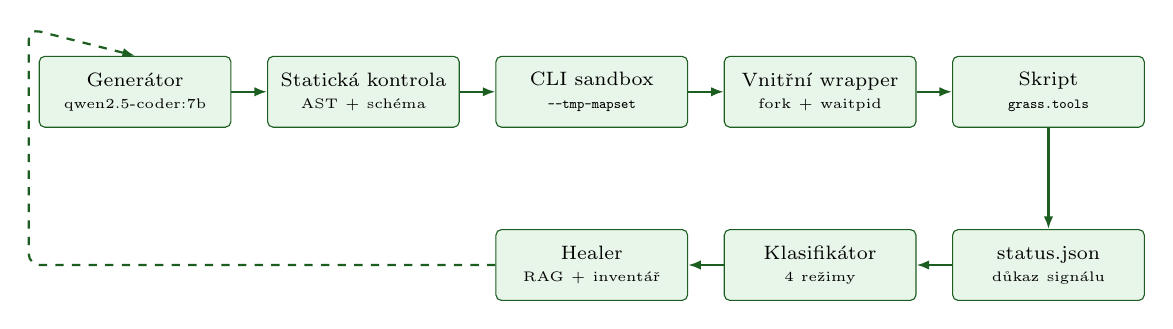
\begin{tikzpicture}[
      font=\scriptsize,
      box/.style={draw=grassdark, fill=grasslight, rounded corners=2pt,
                  align=center, minimum height=9mm, text width=2.2cm},
      arr/.style={-{Latex[length=1.6mm]}, thick, draw=grassdark}
    ]
    \node[box] (gen)      at (0,0)    {Generátor\\{\tiny qwen2.5-coder:7b}};
    \node[box] (static)   at (2.9,0)  {Statická kontrola\\{\tiny AST + schéma}};
    \node[box] (sandbox)  at (5.8,0)  {CLI sandbox\\{\tiny \texttt{-{}-tmp-mapset}}};
    \node[box] (inner)    at (8.7,0)  {Vnitřní wrapper\\{\tiny fork + waitpid}};
    \node[box] (script)   at (11.6,0) {Skript\\{\tiny \texttt{grass.tools}}};

    \draw[arr] (gen) -- (static);
    \draw[arr] (static) -- (sandbox);
    \draw[arr] (sandbox) -- (inner);
    \draw[arr] (inner) -- (script);

    \node[box] (status)   at (11.6,-2.2) {status.json\\{\tiny důkaz signálu}};
    \node[box] (classify) at (8.7,-2.2)  {Klasifikátor\\{\tiny 4 režimy}};
    \node[box] (heal)     at (5.8,-2.2)  {Healer\\{\tiny RAG + inventář}};

    \draw[arr] (script) -- (status);
    \draw[arr] (status) -- (classify);
    \draw[arr] (classify) -- (heal);

    \draw[arr, dashed, rounded corners=4pt]
      (heal.west) -- (-1.35,-2.2) -- (-1.35,0.8) -- (gen.north);
  \end{tikzpicture}

  \vspace{4mm}
  \begin{block}{Jak číst diagram}
    Plná šipka je tok jednoho pokusu; čárkovaná šipka je opravný cyklus.
    Každý uzel má na následujících osmi slidech vlastní vysvětlení: roli,
    mechanismus a důkaz.
  \end{block}
\end{frame}

\begin{frame}[t]{Uzel 1: Generátor}
  \small
  \begin{columns}[T,onlytextwidth]
    \begin{column}{0.49\textwidth}
      \begin{block}{Role}
        \begin{itemize}
          \item Lokální model \texttt{qwen2.5-coder:7b} přes Ollama.
          \item Generuje první pokus i opravy jako Python skript.
          \item Nemá přístup k internetu ani ke stavu verifieru.
        \end{itemize}
      \end{block}
    \end{column}
    \begin{column}{0.49\textwidth}
      \begin{block}{Vstupy a výstupy}
        \begin{itemize}
          \item Vstup: zadání + dohledané dokumenty + inventář map.
          \item Výstup: pouze spustitelný Python (Zero-Chat).
          \item Cílové řešení a očekávané výstupy nejsou v promptu.
        \end{itemize}
      \end{block}
    \end{column}
  \end{columns}

  \begin{exampleblock}{Blok inventáře v promptu}
    \texttt{\#\#\# Available Dataset Maps}\\
    \texttt{These are the ONLY maps that exist in this dataset.}
  \end{exampleblock}

  \begin{alertblock}{Proč je uzel rizikový}
    Generování je stochastické. Statická validita 90\,\% neznamená
    spustitelnost; první pokus uspěje jen u 25\,\% případů.
  \end{alertblock}
\end{frame}

\begin{frame}[t]{Uzel 2: Statická kontrola}
  \small
  \begin{block}{Role}
    Kontrola před spuštěním: parsování AST, validace schématu a vynucení
    rozhraní \texttt{grass.tools}. Odmítne neparsovatelný kód, legacy
    \texttt{grass.script}, shell i řetězená volání.
  \end{block}

  \begin{columns}[T,onlytextwidth]
    \begin{column}{0.49\textwidth}
      \begin{block}{Co se kontroluje}
        \begin{itemize}
          \item Syntaktická správnost Pythonu.
          \item Pouze \texttt{from grass.tools import Tools}.
          \item Žádné \texttt{run\_command}, \texttt{subprocess} ani \texttt{os.system}.
          \item Zero-Chat: žádné Markdown bloky ani próza.
        \end{itemize}
      \end{block}
    \end{column}
    \begin{column}{0.49\textwidth}
      \begin{block}{Co statická kontrola nezachytí}
        \begin{itemize}
          \item Dynamické chyby až při běhu: chybějící mapa, parametry, region.
          \item Statická validita 90\,\% vs.\ Pass@1 25\,\%.
        \end{itemize}
      \end{block}
    \end{column}
  \end{columns}

  \begin{alertblock}{Důkaz}
    Integrační smoke testy přijímají správný skript a odmítají neparsovatelný
    kód, legacy rozhraní i řetězená volání.
  \end{alertblock}
\end{frame}

\begin{frame}[t]{Uzel 3: CLI sandbox}
  \small
  \begin{block}{Role}
    Primární spuštění:
    \texttt{grass -{}-tmp-mapset \textless dataset\textgreater{} -{}-exec python3}.
    Každý pokus dostane dočasný mapset a vlastní scratch adresář.
  \end{block}

  \begin{columns}[T,onlytextwidth]
    \begin{column}{0.49\textwidth}
      \begin{block}{Izolace běhu}
        \begin{itemize}
          \item Dočasný mapset \texttt{-{}-tmp-mapset}.
          \item Neprivilegovaný uživatel \texttt{grader}.
          \item Časový limit 120\,s; \texttt{killpg} ukončí celou skupinu.
          \item Úklid \texttt{tmp\_*} a \texttt{TMPDIR}.
        \end{itemize}
      \end{block}
    \end{column}
    \begin{column}{0.49\textwidth}
      \begin{block}{Trvalá data}
        \begin{itemize}
          \item Zákaz zápisu \texttt{chmod -w} na \texttt{PERMANENT}.
          \item SHA-256 hash před a po běhu (SC-002).
          \item Nulový počet zanechaných scratch složek (SC-004).
        \end{itemize}
      \end{block}
    \end{column}
  \end{columns}

  \begin{alertblock}{\texttt{-{}-tmp-mapset} není bezpečnostní hranice}
    Skript může přepnout mapset a zapisovat do něj. Skutečnou izolaci tvoří
    práva na souborovém systému a kontrola hashe.
  \end{alertblock}
\end{frame}

\begin{frame}[t]{Uzel 4: Vnitřní wrapper}
  \small
  \begin{block}{Role}
    \texttt{inner\_wrapper.py} spouští potomka přes \texttt{fork} a
    \texttt{waitpid} a zapisuje \texttt{status.json}. Cílem je rozlišit pád na
    úrovni C od explicitního \texttt{sys.exit(245)}.
  \end{block}

  \begin{columns}[T,onlytextwidth]
    \begin{column}{0.49\textwidth}
      \begin{block}{Co wrapper zachytí}
        \begin{itemize}
          \item Exit kód a jméno signálu (\texttt{SIGSEGV}, \texttt{SIGABRT}).
          \item Výstup na stdout a stderr.
          \item Konec potomka nezávisle na navazujících procesech.
        \end{itemize}
      \end{block}
    \end{column}
    \begin{column}{0.49\textwidth}
      \begin{block}{Proč nestačí exit kód}
        \begin{itemize}
          \item Kód 245 může znamenat pád i vědomé ukončení.
          \item Bez signálu nelze pád spolehlivě klasifikovat.
          \item \texttt{status.json} je jediný zdroj pravdy.
        \end{itemize}
      \end{block}
    \end{column}
  \end{columns}

  \begin{alertblock}{Důkaz}
    Test se záměrným segfaultem zapíše \texttt{outcome: crashed} a
    \texttt{signal\_name: SIGSEGV}; nevychází přitom z kódu 245.
  \end{alertblock}
\end{frame}

\begin{frame}[t]{Uzel 5: Generovaný skript}
  \small
  \begin{block}{Role}
    Spustitelný Python, který volá pouze moderní \texttt{grass.tools}. Skript
    se ukládá jako artefakt a je znovu použitelný pro audit a reprodukci.
  \end{block}

  \begin{columns}[T,onlytextwidth]
    \begin{column}{0.49\textwidth}
      \begin{block}{Povoleno}
        \begin{itemize}
          \item \texttt{from grass.tools import Tools}.
          \item Volání typu \texttt{tools.r\_slope\_aspect(...)}.
          \item Čistý Python bez Markdownu a prózy.
        \end{itemize}
      \end{block}
    \end{column}
    \begin{column}{0.49\textwidth}
      \begin{block}{Zakázáno}
        \begin{itemize}
          \item \texttt{grass.script.run\_command}.
          \item \texttt{subprocess}, \texttt{os.system}, shell.
          \item Řetězená volání a legacy rozhraní.
        \end{itemize}
      \end{block}
    \end{column}
  \end{columns}

  \begin{alertblock}{Důkaz}
    SC-010 skenuje uložené artefakty a selže při jakémkoli zakázaném volání.
  \end{alertblock}
\end{frame}

\begin{frame}[t]{Uzel 6: \texttt{status.json}}
  \small
  \begin{block}{Role}
    Strojově čitelný důkaz o průběhu pokusu: výsledek, exit kód, signál a
    zachycený výstup. Klasifikátor z něj určuje režim selhání.
  \end{block}

  \begin{table}
    \centering
    \begin{tabular}{@{}lll@{}}
      \toprule
      \textbf{Outcome} & \textbf{Význam} & \textbf{Režim} \\
      \midrule
      \texttt{executed\_ok} & skript doběhl s kódem 0 & úspěch \\
      \texttt{runtime\_failed} & běh skončil chybou & dle stderr \\
      \texttt{crashed} & signál na úrovni C & \texttt{general\_exception} \\
      \texttt{timeout} & překročen limit 120\,s & \texttt{general\_exception} \\
      \bottomrule
    \end{tabular}
  \end{table}

  \begin{alertblock}{Proč samostatný soubor}
    Exit kód sám nerozliší pád a vědomé ukončení. \texttt{status.json} zachová
    signál i kontext pro reprodukovatelnou klasifikaci.
  \end{alertblock}
\end{frame}

\begin{frame}[t]{Uzel 7: Klasifikátor}
  \footnotesize
  \begin{block}{Role}
    Přiřadí každému selhanému pokusu právě jeden ze čtyř režimů. Pořadí je
    pevné, klasifikace je deterministická a idempotentní; žádné selhání nesmí
    zůstat nezařazené.
  \end{block}

  \textbf{Precedence:} \texttt{unknown\_method} $\rightarrow$
  \texttt{missing\_input} $\rightarrow$ \texttt{schema\_misuse} $\rightarrow$
  \texttt{general\_exception}.

  \begin{table}
    \centering
    \begin{tabular}{@{}p{3.1cm}p{7.0cm}p{1.5cm}@{}}
      \toprule
      \textbf{Režim} & \textbf{Typický signál} & \textbf{Počet} \\
      \midrule
      \texttt{missing\_input} & mapa nebo soubor neexistuje & 31 \\
      \texttt{schema\_misuse} & chybějící nebo neplatný parametr & 17 \\
      \texttt{unknown\_method} & neznámý nástroj nebo metoda & 0 \\
      \texttt{general\_exception} & pád, timeout, neošetřená chyba & 35 \\
      \bottomrule
    \end{tabular}
  \end{table}

  \begin{alertblock}{Důkaz}
    112 testů klasifikátoru pokrývá precedence, lokalizované chyby a
    idempotenci; všech 83 selhaných pokusů je klasifikováno (SC-005).
  \end{alertblock}
\end{frame}

\begin{frame}[t]{Uzel 8: Healer (opravný cyklus)}
  \footnotesize
  \begin{columns}[T,onlytextwidth]
    \begin{column}{0.49\textwidth}
      \begin{block}{Role a mechanismus}
        \begin{itemize}
          \item Max. 2 opakování; každé selhání spotřebuje jeden pokus.
          \item RAG nad 543 nástroji + cílený dotaz na selhávající nástroj.
          \item Opravný prompt nese 4 prvky: chybu, dokumentaci, kód a inventář.
          \item Zastaví se při úspěchu nebo vyčerpání rozpočtu.
        \end{itemize}
      \end{block}
    \end{column}
    \begin{column}{0.49\textwidth}
      \begin{block}{Ukotvení v inventáři (FR-012a/b)}
        \begin{itemize}
          \item \texttt{inventory.py} čte \texttt{PERMANENT/cellhd} a
                \texttt{vector} přímo.
          \item Bez GRASS relace; max. 80 map; záložní \texttt{g.list}.
          \item Inventář jde do 1. pokusu i do všech oprav.
          \item Nečitelné mapy se vynechají, nikdy se nevymýšlejí.
        \end{itemize}
      \end{block}
    \end{column}
  \end{columns}

  \begin{alertblock}{Naměřený dopad a limit}
    \texttt{missing\_input}: 56 $\rightarrow$ 31 ($-$45\,\%); healing gain
    +12,5\,p.\,b. Opakovaná stejná selhání však dominují (49 z 56); další
    zlepšení vyžaduje ukotvení parametrů, ne jen více opakování.
  \end{alertblock}
\end{frame}

% ============================================================================
%  4. VÝSLEDKY A ANALÝZA
% ============================================================================
\section{Výsledky a analýza}

\begin{frame}[t]{Hlavní výsledky: statická vs. dynamická validita}
  \small
  \begin{table}
    \centering
    \begin{tabular}{@{}lrr@{}}
      \toprule
      \textbf{Měření} & \textbf{Případy} & \textbf{Úspěšnost} \\
      \midrule
      Gate 1 statická validita (baseline) & 36/40 & 90,0\,\% \\
      Gate 2 Pass@1 (zero-shot) & 10/40 & 25,0\,\% \\
      Gate 2 Pass@Healed (max. 2 opakování) & 15/40 & 37,5\,\% \\
      \midrule
      \textbf{Nárůst díky opravám (healing gain)} & \textbf{+5 případů}
        & \textbf{+12,5\,p.\,b.} \\
      \bottomrule
    \end{tabular}
  \end{table}

  \begin{alertblock}{Klíčový poznatek}
    Statická analýza AST a validace schématu jsou slabými ukazateli
    spustitelnosti v GIS: statická validita dosahuje 90,0\,\%, ale pouze
    25,0\,\% skriptů reálně proběhne na první pokus.
  \end{alertblock}

  \begin{exampleblock}{Přínos self-healingu}
    +12,5 procentního bodu (+50\,\% relativně): 5 dodatečných případů opraveno
    v rámci limitu 2 opakování.
  \end{exampleblock}

  {\footnotesize Pass@Healed měří spustitelnost, nikoli geografickou správnost
  (FR-021, SC-014).}
\end{frame}

\begin{frame}[t]{Odhalení skrytých chyb}
  \small
  \begin{columns}[T,onlytextwidth]
    \begin{column}{0.46\textwidth}
      \begin{table}
        \centering
        \begin{tabular}{@{}lr@{}}
          \toprule
          \textbf{Režim selhání} & \textbf{Pokusy} \\
          \midrule
          \texttt{general\_exception} & 35 \\
          \texttt{missing\_input} & 31 \\
          \texttt{schema\_misuse} & 17 \\
          \midrule
          \textbf{Celkem} & \textbf{83} \\
          \bottomrule
        \end{tabular}
      \end{table}

      {\scriptsize \texttt{unknown\_method}: 0 výskytů v tomto běhu.}
    \end{column}

    \begin{column}{0.52\textwidth}
      \begin{block}{Vyřešeno: halucinace vrstev}
        \texttt{missing\_input} klesl z 56 na 31 ($-$45\,\%) po zavedení
        inventáře map.
      \end{block}

      \begin{block}{Odhaleno: hlubší chyby}
        \texttt{general\_exception} vzrostl z 10 na 35, což odkrylo:
        \begin{itemize}
          \item \texttt{v.to.rast} bez parametru \texttt{column=}
          \item \texttt{d.rast} bez monitoru \texttt{d.mon}
          \item Nesoulad nastavení regionu (\texttt{g.region})
        \end{itemize}
      \end{block}
    \end{column}
  \end{columns}

  \begin{alertblock}{Interpretace výsledků}
    Úspěšnost nevzrostla skokově, protože oprava názvu vrstvy odkryla další
    chybový stupeň. Jde o diagnostický pokrok, který předchází celkovému úspěchu.
  \end{alertblock}
\end{frame}

\begin{frame}[t]{Přechody mezi režimy selhání}
  \small
  \begin{table}
    \centering
    \begin{tabular}{@{}llr@{}}
      \toprule
      \textbf{Přechod} & \textbf{Význam přechodu} & \textbf{Počet} \\
      \midrule
      \texttt{general\_exception} $\rightarrow$ \texttt{general\_exception}
        & Přetrvává stejná chyba & 21 \\
      \texttt{missing\_input} $\rightarrow$ \texttt{missing\_input}
        & Přetrvává chybějící vstup & 20 \\
      \texttt{schema\_misuse} $\rightarrow$ \texttt{schema\_misuse}
        & Přetrvává chyba schématu & 8 \\
      \texttt{schema\_misuse} $\rightarrow$ \texttt{general\_exception}
        & Odhalena hlubší chyba & 3 \\
      \texttt{general\_exception} $\rightarrow$ \texttt{success}
        & Úspěšně opraveno & 1 \\
      \texttt{schema\_misuse} $\rightarrow$ \texttt{success}
        & Úspěšně opraveno & 1 \\
      \bottomrule
    \end{tabular}
  \end{table}

  \begin{alertblock}{Vyhodnocení}
    Dominují opakovaná selhání ve stejném režimu (49 z 56).
  \end{alertblock}

  \begin{block}{Důsledek pro další vývoj}
    Opravné prompty vyžadují silnější ukotvení na úrovni parametrů a schémat
    nástrojů.
  \end{block}
\end{frame}

\begin{frame}[t]{Výkonnost běhu a testovací sada}
  \small
  \begin{columns}[T,onlytextwidth]
    \begin{column}{0.50\textwidth}
      \begin{table}
        \centering
        \begin{tabular}{@{}lr@{}}
          \toprule
          \textbf{Metrika} & \textbf{Hodnota} \\
          \midrule
          Hodnocené případy & 40/40 \\
          Hardware & Colab Tesla T4 (15\,GB) \\
          Celkový čas & 16,8 min \\
          Tokeny na úspěch & $\sim$7{,}356 \\
          Sada testů & 250 testů \\
          Verze GRASS GIS & 8.5.0 \\
          \bottomrule
        \end{tabular}
      \end{table}
    \end{column}

    \begin{column}{0.48\textwidth}
      \begin{block}{Správa a řízení testů}
        \begin{itemize}
          \item Jednotkové, integrační a kontraktní testy.
          \item Neprivilegovaný účet \texttt{grader}.
          \item Příprava prostředí přes \texttt{run\_remote.sh}.
        \end{itemize}
      \end{block}

      \begin{block}{Deterministické výkazy}
        Parametr \texttt{-{}-report-only} vygeneruje zprávu z uložených dat bez
        volání LLM nebo GRASS.
      \end{block}
    \end{column}
  \end{columns}

  \begin{exampleblock}{Integrita výkaznictví}
    Generování zpráv ověřeno jako bajtově identické při opakovaném zpracování
    (SC-013).
  \end{exampleblock}
\end{frame}

\begin{frame}[t]{Co obsahuje sada 250 testů}
  \footnotesize
  \begin{table}
    \centering
    \begin{tabular}{@{}p{4.2cm}p{7.0cm}r@{}}
      \toprule
      \textbf{Oblast} & \textbf{Co ověřuje} & \textbf{Počet} \\
      \midrule
      Klasifikace a chyby
        & 4 režimy, precedence, lokalizace, idempotence & 116 \\
      Self-healing a ukotvení
        & 4 prvky opravy, Zero-Chat, inventář, cílený dotaz & 45 \\
      Vykonávání a izolace
        & segfault, timeout, PERMANENT hash, scratch, offline & 21 \\
      Kontrakty a perzistence
        & přepínače CLI, fixtures, atomický zápis, obnovení & 58 \\
      Reportování
        & Pass@1/Healed, počty režimů, přechody, výhrada ke korektnosti & 15 \\
      \midrule
      \textbf{Celkem v aktuální kolekci} & & \textbf{255} \\
      \bottomrule
    \end{tabular}
  \end{table}

  \begin{block}{Jak testy vznikají}
    Jednotkové, integrační a kontraktní testy přes \texttt{pytest}; běh na Colab
    s GRASS GIS 8.5.0 pod neprivilegovaným uživatelem \texttt{grader}.
  \end{block}

  \begin{alertblock}{Poznámka k počtu}
    Reportovaný běh Gate 2: 250 testů. Aktuální kolekce v repozitáři: 255 testů
    (5 parametrizovaných případů navíc); před publikací sjednotit.
  \end{alertblock}
\end{frame}

% ============================================================================
%  5. DISKUZE A OTÁZKY
% ============================================================================
\section{Diskuze a otázky}

\begin{frame}[t]{Diskuze: co Gate 2 potvrzuje}
  \small
  \begin{block}{1. Rozdíl oproti statické analýze je potvrzen}
    Statická validita 90,0\,\% vs.\ spustitelnost na 1. pokus 25,0\,\%.
    Syntaxe a schéma nezaručují spuštění v prostředí.
  \end{block}

  \vspace{2mm}

  \begin{block}{2. Ukotvení a self-healing mají měřitelný přínos}
    Ukotvení v inventáři snížilo \texttt{missing\_input} z 56 na 31; ohraničený
    self-healing přidal +12,5\,p.\,b. (+50\,\% relativně).
  \end{block}

  \vspace{2mm}

  \begin{block}{3. Bezpečnost spuštění je prokázána}
    Bezhlavý CLI sandbox, izolace procesních skupin, nezměněný hash
    \texttt{PERMANENT} a nulové úniky dočasných adresářů.
  \end{block}
\end{frame}

\begin{frame}[t]{Možnosti dalšího postupu}
  \small
  \begin{table}
    \centering
    \begin{tabular}{@{}p{3.8cm}p{4.2cm}p{5.0cm}@{}}
      \toprule
      \textbf{Možnost} & \textbf{Přínos} & \textbf{Náklady a rizika} \\
      \midrule
      Ukotvení parametrů v RAG
        & Cílení na chybějící \texttt{column=}, region a monitory
        & Nízké náklady; riziko kvality vyhledávání \\
      Větší modely (14B/32B)
        & Testování škálování nad rámec 7B
        & Vysoké nároky na GPU a čas \\
      Konsolidace a dokumentace
        & Shromáždění výsledků z Gate 1 a Gate 2
        & Nízké náklady; odkládá další vývoj \\
      \bottomrule
    \end{tabular}
  \end{table}

  \begin{block}{Doporučené pořadí diskuse}
    \begin{enumerate}
      \item Ukotvení parametrů: nejvyšší přínos proti odhalené vrstvě
            \texttt{general\_exception}.
      \item Škálování modelů: pouze pokud rozdělení chyb ospravedlňuje
            operativní náklady.
      \item Konsolidace výstupů: ukotvení ověřeného přínosu Gate 2.
    \end{enumerate}
  \end{block}
\end{frame}

\begin{frame}[t]{Stopa důkazů a reprodukovatelnost}
  \small
  \begin{table}
    \centering
    \footnotesize
    \begin{tabular}{@{}p{5.0cm}p{8.0cm}@{}}
      \toprule
      \textbf{Artefakt} & \textbf{Obsah} \\
      \midrule
      \texttt{benchmarks/execution\_report.md}
        & Hlavní metriky, režimy selhání, přechody, náklady na tokeny \\
      \texttt{benchmarks/leakage\_report.md}
        & Audit kontaminace: Jaccard, n-gramy, označené případy \\
      \texttt{grass\_agent/}
        & Vykonávání, \texttt{inner\_wrapper.py}, inventář, self-healing \\
      \texttt{specs/}
        & Specifikace, plán, výzkum, datový model, kontrakty \\
      \texttt{tests/} + \texttt{run\_remote.sh}
        & 250 testů v reportovaném běhu a příprava prostředí v Colab \\
      \bottomrule
    \end{tabular}
  \end{table}

  \begin{block}{Jak prezentaci ověřit}
    Začněte výkazem exekuce, potom auditem úniku a nakonec kontrakty izolace.
    Všechna čísla mají původ v uloženém artefaktu nebo v zadání konzultace.
  \end{block}
\end{frame}

\begin{frame}[t]{Otázky a diskuze}
  \begin{block}{K diskuzi}
    \begin{itemize}
      \item Je navržená izolace dostatečná pro obhajobu, nebo je třeba ji
            rozšířit?
      \item Má Gate 3 prioritizovat parametrické RAG ukotvení, nebo škálování
            modelu?
      \item Jak prezentovat rozdíl mezi spustitelností a geografickou
            správností?
    \end{itemize}
  \end{block}

  \vspace{6mm}
  \begin{center}
    \Large\color{grassdark}\textbf{Děkuji za pozornost.}
  \end{center}
\end{frame}

\end{document}
